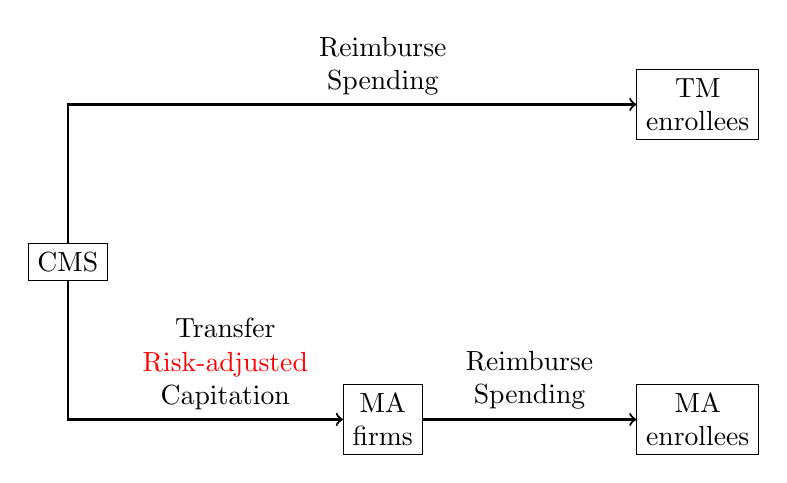
\begin{tikzpicture}
    \node[draw] (CMS) at (0,2) {CMS};
    \node[draw, align=center] (TM) at (8,4) {TM \\ enrollees};
    \node[draw, align=center] (MA) at (8,0) {MA \\ enrollees};
    \node[draw, align=center] (MAf) at (4,0) {MA \\ firms};

    \draw[->, thick] (CMS.north) |- (TM.west);
    \draw[->, thick] (CMS.south) |- (MAf.west);
    \draw[->, thick] (MAf.east) -- (MA.west) node[midway, above, align=center] {Reimburse \\ Spending};

    \node[above, align=center] at (4,4) {Reimburse \\ Spending};
    \node[above, align=center] at (2,0) {Transfer \\ \textcolor{red}{Risk-adjusted} \\ Capitation};
\end{tikzpicture}